\documentclass[12pt]{article}
% Packages
\usepackage[margin=1in]{geometry}
\usepackage{setspace}
\usepackage{graphicx}
\usepackage{amsmath}
\usepackage{amssymb}
\usepackage{booktabs}
\usepackage{natbib}
\usepackage{hyperref}
\usepackage{titlesec}
\usepackage{overpic}
\usepackage{float}
\usepackage{subcaption}
\usepackage{placeins}
\usepackage{tikz}
\usepackage[percent]{overpic}

\onehalfspacing

\setcounter{secnumdepth}{0}


\title{\textbf{Early-life unpredictability modulates uncertainty-adaptive planning in a structured foraging task in humans.}}

\author{
Yifan Zhang$^{1,2,*}$ \and
Yifei Chen$^{3,*}$ \and
X. Roger Chen$^{1} \and 
Nora C. Harhen$^{4}$ \and
Laura A. Glynn$^{5} \and
Elysia P. Davis$^{6} \and
Daniel A. Stout$^{7,8}$ \and
Aaron M. Bornstein$^{1,2,9,10}}

\date{}

\begin{document}

\maketitle

\begin{flushleft}
\small
$^{1}$ Department of Cognitive Sciences, University of California, Irvine, CA, USA \\
$^{2}$ Center for Theoretical Behavioral Sciences, University of California, Irvine, CA, USA \\
$^{3}$ Department of Psychology, Princeton University, Princeton, NJ, USA \\
$^{4}$ Department of Psychology, New York University, New York, NY, USA \\
$^{5}$ Department of Psychology, Chapman University, Orange, CA, USA \\
$^{6}$ Department of Psychology, University of Denver, Denver, CO, USA \\
$^{7}$ Department of Psychiatry, University of California, San Diego, CA, USA \\
$^{8}$ Center of Excellence for Stress and Mental Health, Veterans Affairs San Diego Healthcare System, San Diego, CA, USA \\
$^{9}$ Center for the Neurobiology of Learning and Memory, University of California, Irvine, CA, USA \\
$^{10}$ Drury Institute for Translational Depression Discoveries, University of California, Irvine, CA, USA \\[0.5em]
Correspondence: yifaz79@uci.edu
\end{flushleft}



\section*{Abstract}

It has been shown that early-life environments shape how individuals learn and adapt to uncertainty, yet the computational pathways linking early-life unpredictability (ELU) to adult decision-making remain unclear. Here, we combine a structured foraging task with computational modeling to test how ELU influences uncertainty-dependent planning. Participants performed a sequential foraging task requiring continuous trade-offs between exploiting depleting resources and exploring alternatives, alongside assessments of early-life unpredictability (QUIC) and trauma-related symptoms (PCL). We fit a structural learning model in which uncertainty modulates the valuation of leaving a current resource patch via an uncertainty-sensitive discounting parameter. We found that ELU was associated with increased uncertainty weighting. Critically, ELU showed only weak direct associations with overharvesting behavior. Instead, mediation analyses revealed a robust indirect pathway: ELU predicted increased uncertainty weighting, which in turn predicted greater overharvesting relative to the Marginal Value Theorem. This pattern was consistent across environmental conditions, indicating that early-life unpredictability primarily influences behavior through latent computational mechanisms rather than direct behavioral effects. Importantly, although PCL were correlated with uncertainty weighting at the zero-order level, these effects were fully accounted for by shared variance with ELU. In contrast, ELU uniquely predicted uncertainty weighting, clear dissociation between developmental unpredictability and current PTSD symptom severity. Together, our results show that early-life unpredictability shapes adult decision-making by altering how uncertainty is integrated into valuation, rather than directly changing behavior.


\section*{Introduction}

Foraging in natural environments requires balancing the exploitation of known resources against exploration of alternatives. In sequential foraging contexts, this balance is governed by estimates of environmental richness and uncertainty, which together determine when it is advantageous to leave a depleting resource patch. While extensive work has characterized optimal foraging strategies and their neural and computational substrates, less is known about how individual differences—particularly those rooted in early-life experience—shape these decision processes.

Early-life unpredictability (ELU) has been proposed as a critical developmental factor influencing learning and decision-making \citep{harhen2025developmental,decker2025exploration,rachum2025early}. Exposure to unstable or unpredictable environments during development may alter how individuals represent and respond to uncertainty, potentially leading to persistent differences in valuation and action selection. Prior work has linked ELU to altered learning rates, risk preferences, and affective processing, yet a mechanistic account of how ELU influences decision-making in dynamic, temporally extended tasks remains lacking.

One promising framework for addressing this question is to examine how uncertainty is incorporated into the computation of opportunity costs during foraging. In canonical models \citep{charnov1976optimal,sutton1988learning}, decisions to leave a patch depend on a comparison between the expected value of staying and the average reward rate of the environment. However, when environmental structure is uncertain, agents must infer latent dynamics and adjust their decision policies accordingly. This suggests that individual differences in how uncertainty is weighted could lead to systematic variation in foraging behavior.

Here, we combine a sequential foraging paradigm with computational modeling to test the hypothesis that ELU modulates uncertainty-dependent valuation. Participants completed a foraging task in which rewards depleted over time, alongside assessments of early-life unpredictability (QUIC) and trauma-related symptom severity. We developed an adaptive discounting model in which trial-by-trial uncertainty modulates the value of leaving, captured by an uncertainty-weighting parameter.

We hypothesized that individuals with greater ELU would exhibit increased sensitivity to uncertainty, reflected in stronger modulation of decision values by uncertainty. Furthermore, we tested whether this relationship is specific to ELU or can be explained by trauma-related symptom severity. By linking early-life experience to computational parameters governing decision-making, this work aims to provide a mechanistic account of how developmental environments shape adaptive behavior in uncertain and dynamic contexts.


\section*{Materials and Methods}

\subsection*{Participants}

297 participants from Amazon Mechanical Turk (142 females, 144 males, 2 others, 9 unknown; 46.86 ± 0.89 years old) between May 3 and July 2, 2024, using the CloudResearch Approved Group Filter. They received a base payment of \$15.00 for completing the patch-leaving Task, with a potential bonus of up to \$5.00 contingent on performance on two randomly selected planet. Of these participants, 263 filled out the Questionnaire of Unpredictability in Childhood (QUIC), 147 filled out the Life Event Checklist (LEC-5) and the Post-Traumatic Stress Disorder Checklist (PCL-5). 181 completed the Mnemonic Similarity Task (MST) for an additional \$5.00 compensation. The recruitment was limited to participants who (1) had a minimum 95\% approval rate, (2) had completed at least 50 approved tasks, and (3) were located in the United States. Inclusion criteria required that participants (1) passed the instruction quiz with fewer than three attempts, (2) passed both attention checks, (3) had a mean residence time within two standard deviations of the group average, and (4) spent on average at least two digs per planet to ensure sufficient exposure to patch types.

\subsection*{Experiment Setup}

Participants completed an online serial stay–switch foraging task adapted from prior human foraging tasks (e.g. \citep{constantino2015learning}). The primary way in that the task differed from previous work is that it elicited behavior in the presence of multiple patch types \citep{harhen2023overharvesting,harhen2026structure}. Participants were instructed to maximize total reward by traveling between planets and mining space gems across five blocks of fixed duration (6 minutes each), separated by self-paced breaks of up to one minute.

Upon arrival at a new planet (Fig.~\ref{fig:task}A), participants performed an initial dig and received a gem reward sampled from a Gaussian distribution (mean = 100, SD = 5). After each dig, they decided whether to stay on the current planet or leave to travel to a new one. Staying allowed further exploitation of the current resource, whereas leaving incurred a longer travel delay but granted access to a replenished gem mine. Participants had up to 2 seconds to respond; missed responses resulted in a brief timeout.

Temporal costs were structured so that reaction time did not directly affect reward rate. Stay decisions were followed by a 1.5-second delay before reward feedback, with total trial duration held constant. Leave decisions incurred a 10-second travel delay, followed by arrival on a new planet before mining resumed.

Planets differed in richness, defined by the rate at which rewards decayed exponentially with successive digs. Three planet types were used—poor, neutral, and rich—with decay rates sampled from beta distributions producing fast, intermediate, and slow depletion, respectively (Fig.~\ref{fig:task}B).

Environmental structure extended across planets. When traveling to a new planet, there was an 80\% probability that it would be of the same type as the previous planet and a 20\% probability of switching to one of the other two types (Fig.~\ref{fig:task}C). This transition structure was not disclosed to participants.


\begin{figure}[H]
    \centering
    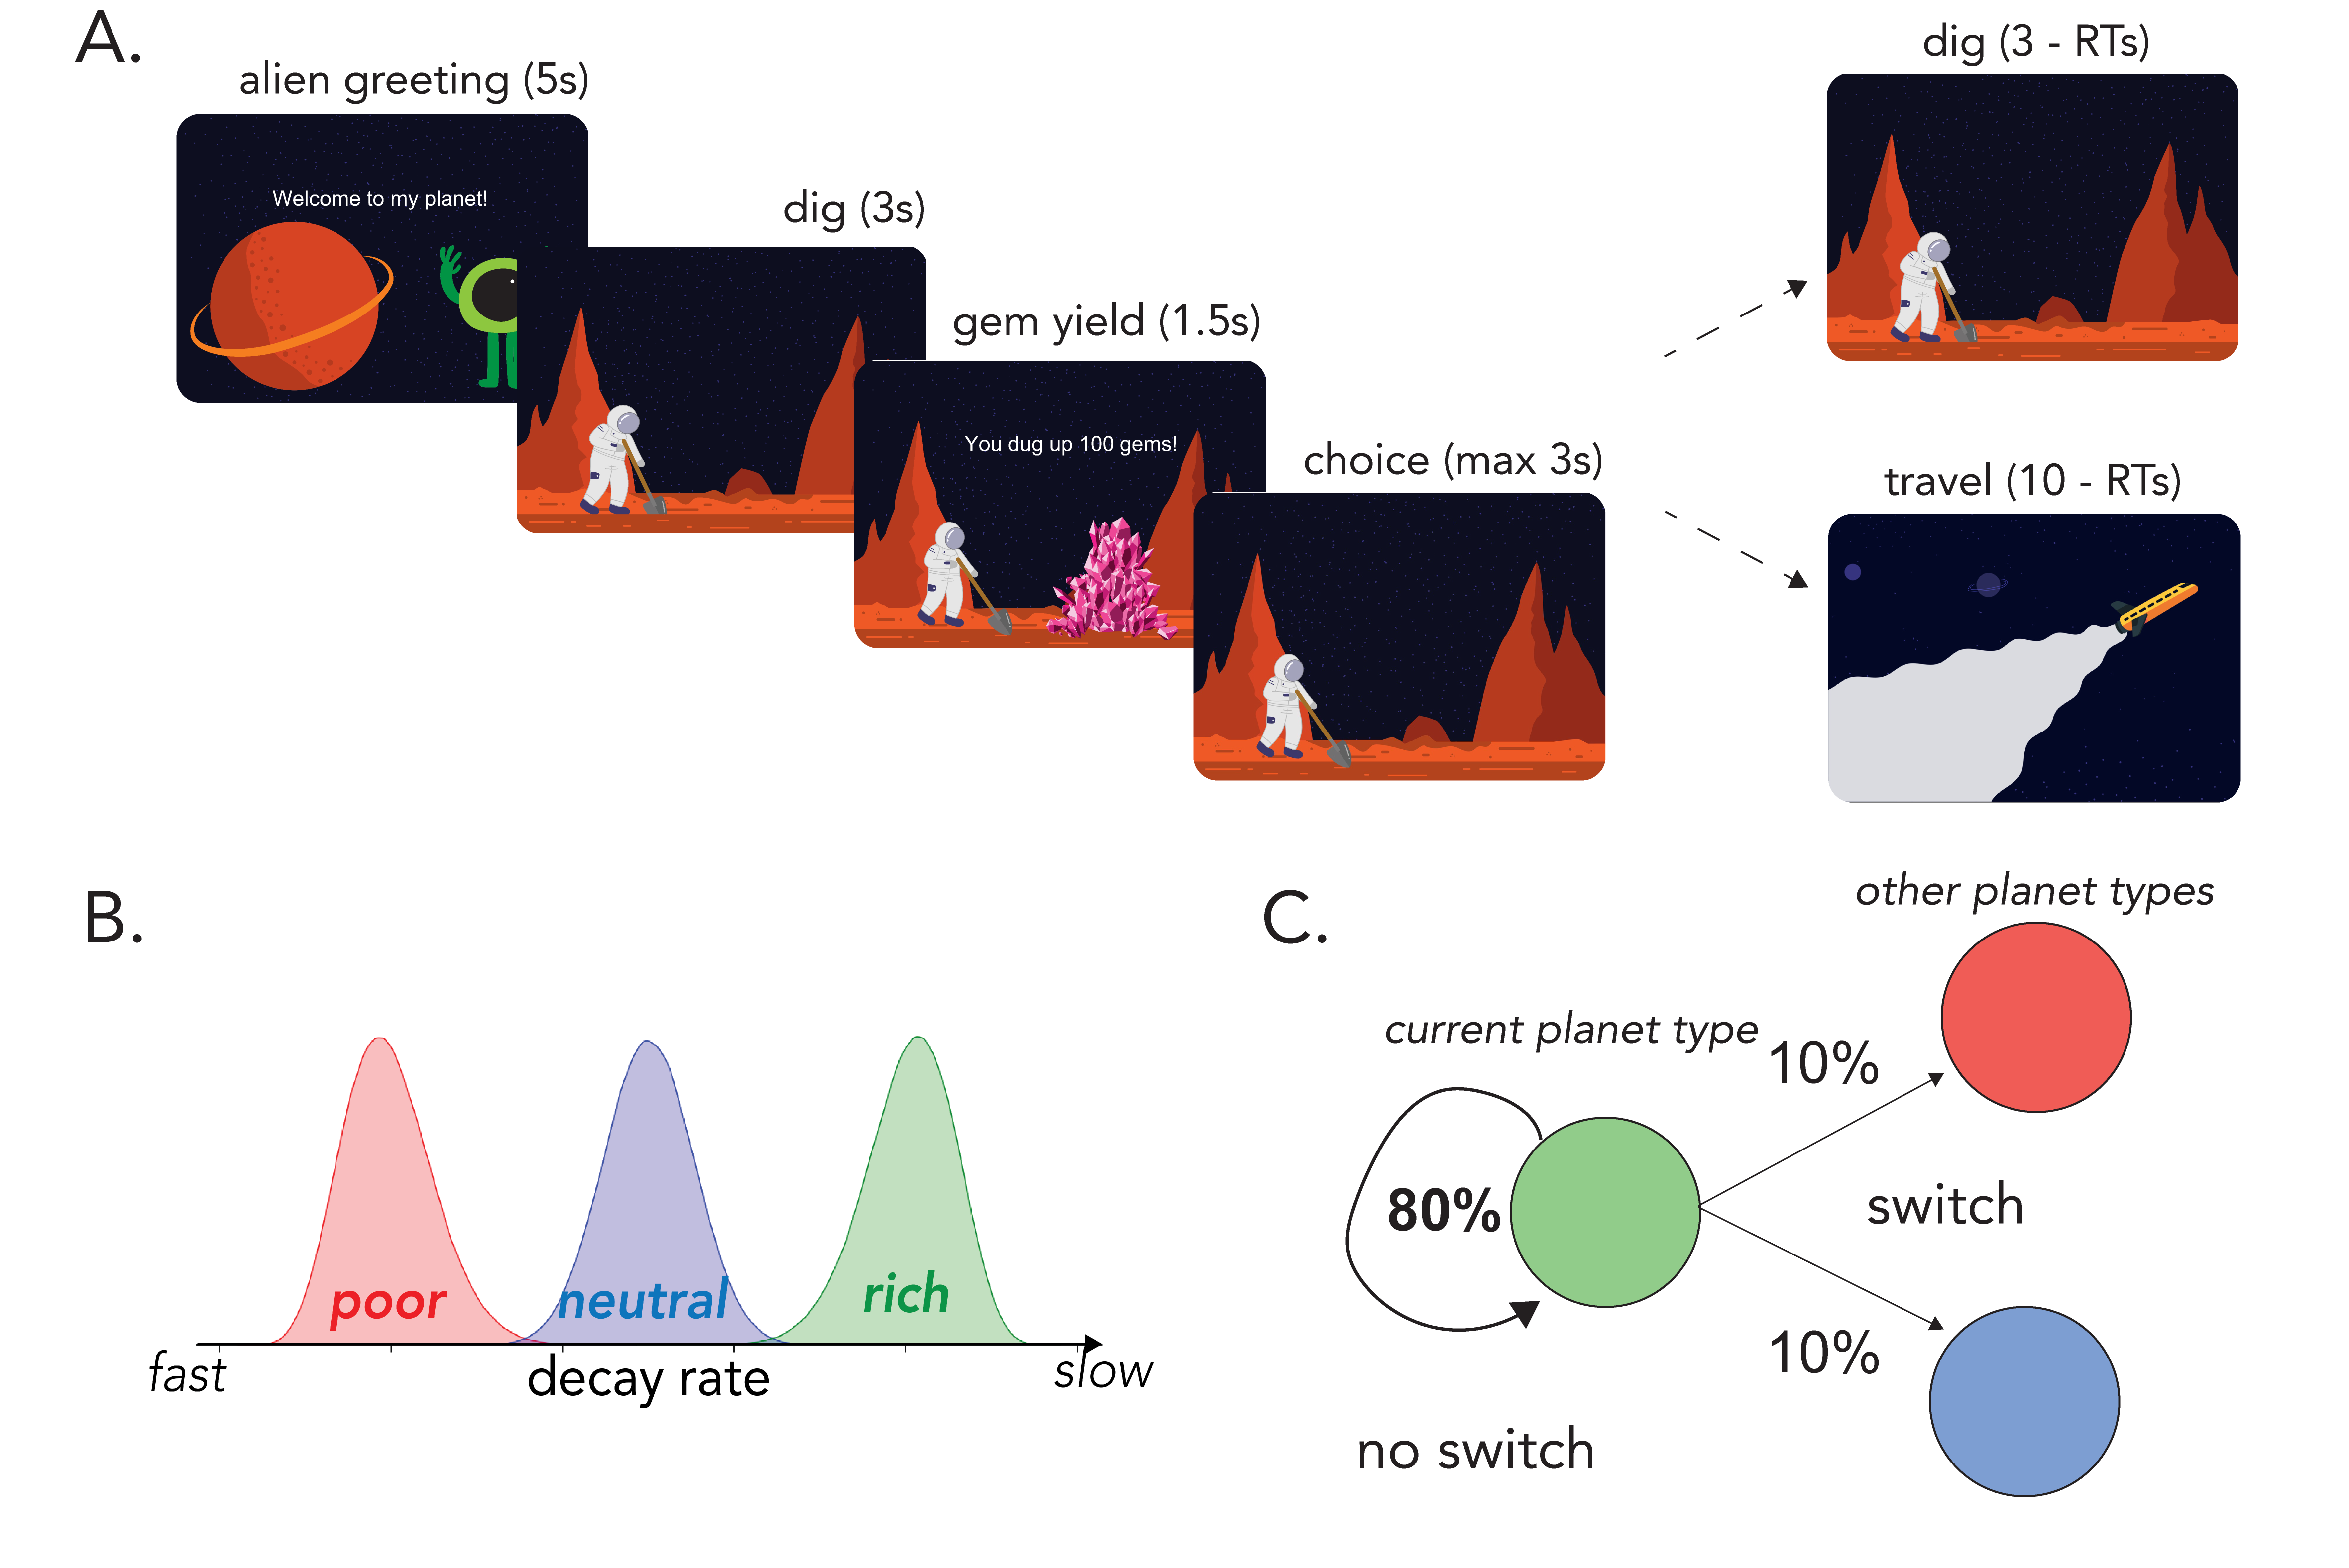
\includegraphics[width=0.75\linewidth]{figure1.png}
    \caption{Planet Foraging Task: (A) Serial stay-switch task. Participants traveled to different planets and mined space gems across five 6-min blocks. On each trial, they had to decide between staying to dig from a depleting gem mine or incurring a time cost to travel to a new planet. (B) Environment structure. Planets varied in their richness or, more specifically, the rate at which they exponentially decayed with each dig. There were three planet types: poor, neutral, and rich—each with its own characteristic distribution over decay rates. (C) Environment dynamics. Planets of a similar type clustered together. A new planet had an 0.8 probability of being the same type as the prior planet (``no switch''). However, there was a 0.2 probability of transitioning or ``switching'' to a planet of a different type.}
    \label{fig:task}
\end{figure}

\subsection*{Optimal Planet Residence Time: Marginal Value Theorem}

We compared participants' planet residence time (PRT; the number of digs performed on the planet) to the optimal residence time prescribed by the Marginal Value Theorem (MVT). The MVT agent assumes perfect knowledge of decay rates and reward history.

The value of staying is:

\[
V_{\text{stay}} = r_t \times d
\]

where \( r_t \) is the previous reward and \( d \) is the decay rate.

The value of leaving is:

\[
V_{\text{leave}} = \frac{r_{\text{total}}}{t_{\text{total}}} \times t_{\text{dig}}
\]

The agent chooses the higher of \( V_{\text{stay}} \) and \( V_{\text{leave}} \).



\subsection*{Questionnaire of Unpredictability in Childhood (QUIC)}

Participants completed the 38-item QUIC \citep{glynn2019measuring}, assessing perceived unpredictability before ages 12 and 18 across five domains: parental involvement and monitoring, parental predictability, parental environment, physical environment, and safety/security. Responses were recorded as “yes,” “no,” or “prefer not to say.” The total score ranges from 0–38, with higher scores indicating greater early-life unpredictability.

To better characterize the latent structure of early-life unpredictability in our sample, we conducted factor analysis on the 38 QUIC items, using a separate 732 individuals’ QUIC responses (278 females, 453 males, 1 other, 36.53 ± 10.99 years old, range 18-70) also collected on Amazon Mechanical Turk from May 2024 to July 2024. All the items (38 in total) were included in the analysis. Maximum likelihood estimation was used for factor extraction, and an oblique rotation (Promax) was selected. Factors were thresholded by eigenvalue > 1. The EFA revealed that there are 6 latent factors. The factor loadings of each factor from each response are presented in Table 1.
 
Factor extraction was performed using exploratory factor analysis with maximum likelihood/principal axis factoring, followed by oblique rotation to allow factors to correlate. Factors were thresholded by eigenvalue > 1.We identified six factors; labels were decided based on manual examination of the questions assigned to each factor (see Supplement, Table 1). 

Items loading onto each factor were grouped accordingly, and factor scores were computed at the individual level by summing responses within each factor. These factor scores were standardized prior to analysis. The five factors were used in subsequent behavioral and computational analyses to examine whether specific dimensions of early-life unpredictability differentially predicted foraging behavior and model-derived parameters.

In addition to the factor-level analyses, we computed the total QUIC score as a global measure of early-life unpredictability to assess broad associations with behavioral and computational outcomes.

\subsection*{Life Event Checklist (LEC-5)}

The LEC-5 assesses lifetime exposure to potentially traumatic events. Participants indicated whether events happened to them, were witnessed, learned about, part of their job, unsure, or did not apply. Total scores (0–34) reflect direct exposure.


\subsection*{Post-Traumatic Stress Disorder Checklist (PCL-5)}

PCL-5 is a 20-item self-report measure of PTSD symptoms that corresponds to the criteria of DSM-5 \citep{wortmann2016psychometric}. Participants rated symptom severity from 0 (“Not at all”) to 4 (“Extremely”). Total scores range from 0–80. We performed a factor analysis using the same procedure as that in QUIC, under which we identified three factors. 


\subsection*{Mnemonic Similarity Task (MST)}

The Mnemonic Similarity Task \citep{stark2019mnemonic} assesses the ability of participants to correctly identify similar (``Lure''), as opposed to repeated or entirely new (``Foil''), image stimuli in a continuous-recognition style task. During encoding, participants categorized 128 objects as indoor or outdoor. During retrieval, they classified 192 objects as old, similar, or new. The lure discriminant index (LDI) was computed as:

\[
LDI = P(\text{“similar”|Lure}) - P(\text{“similar”|Foil})
\]


\begin{figure}
    \centering
    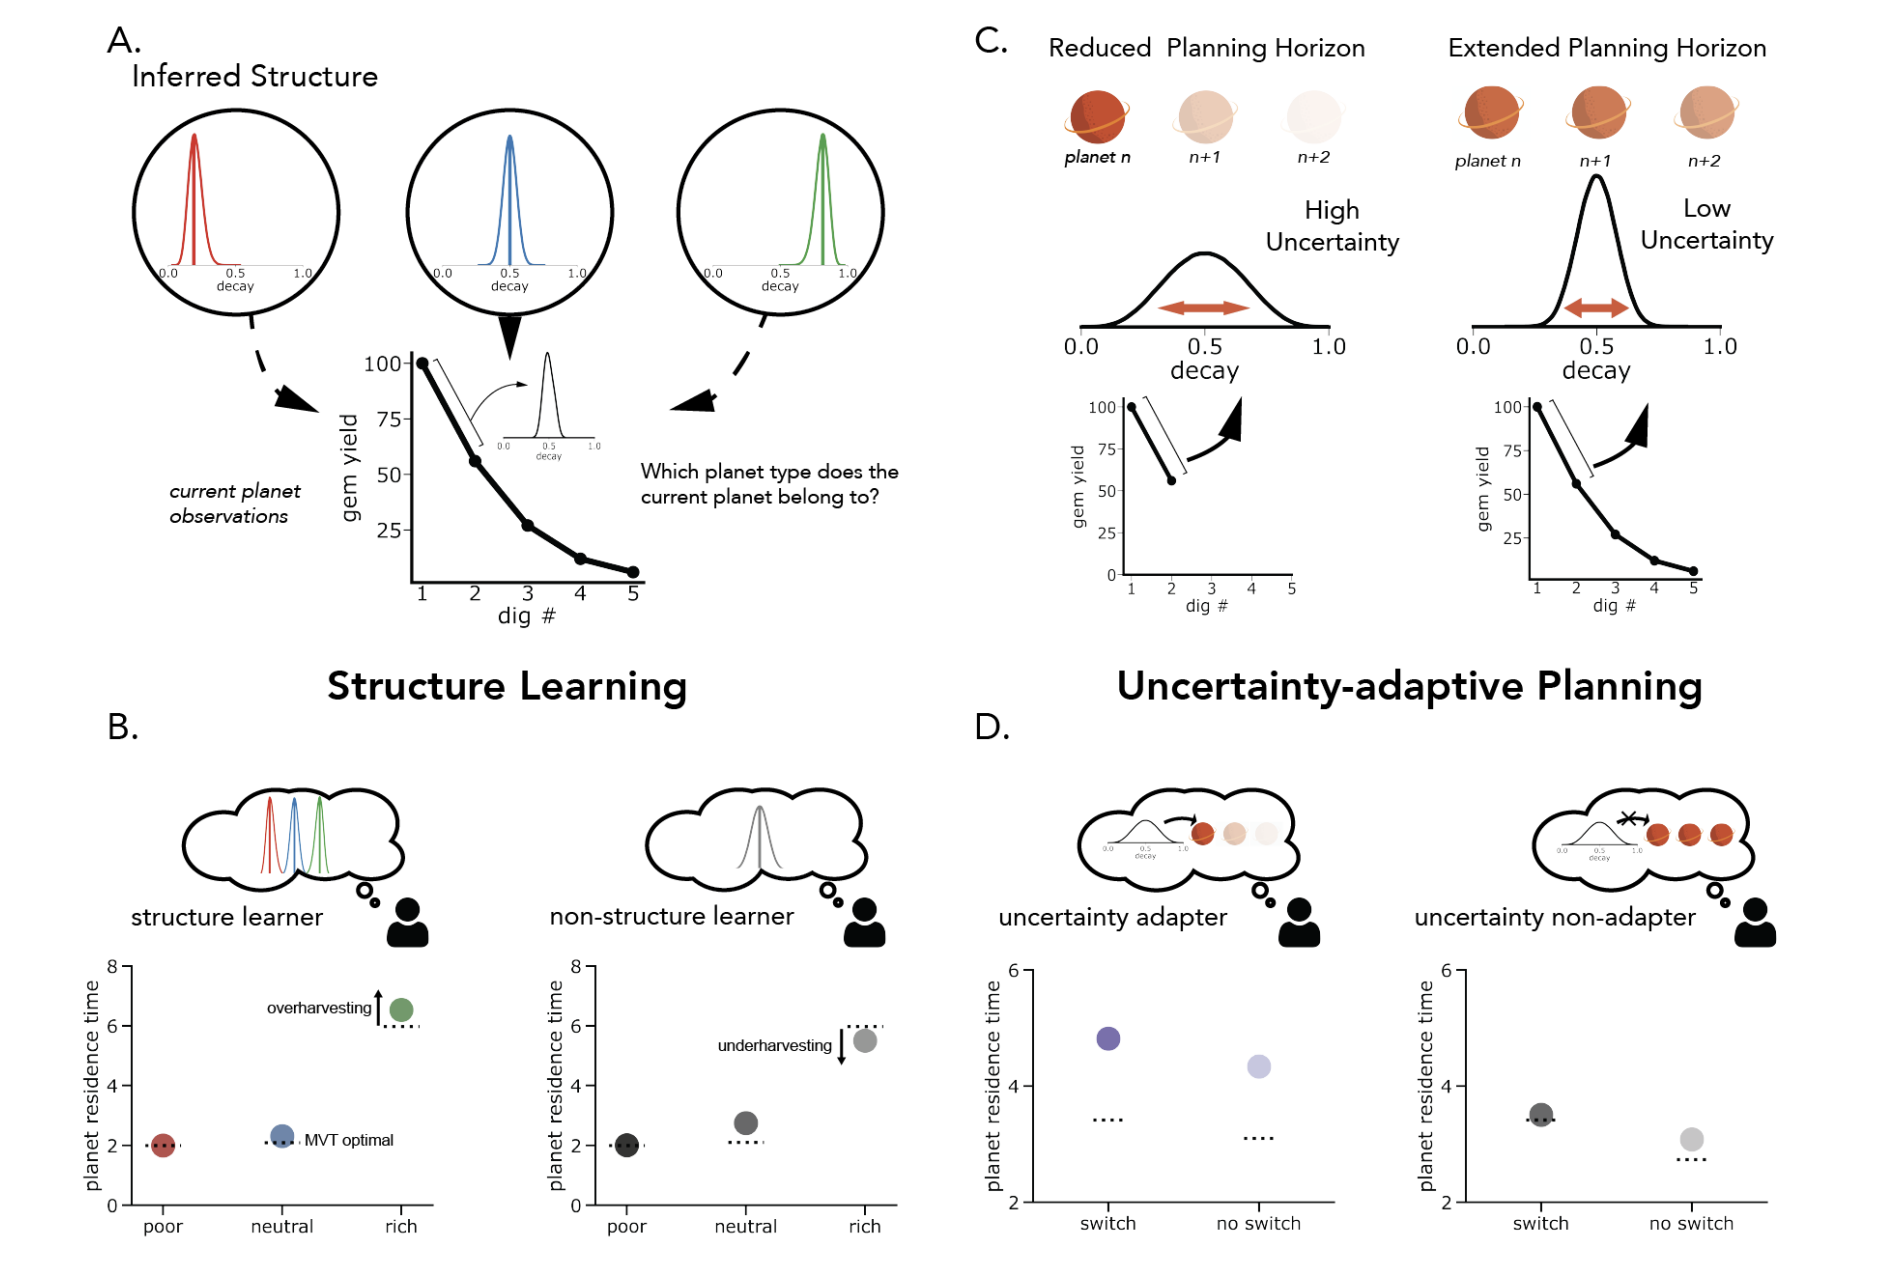
\includegraphics[width=1\linewidth]{figure2.png}
    \caption{\textbf{Computational framework for structure learning and uncertainty-dependent planning.}
    (A) The forager performs two concurrent inferences: estimating the latent type of the current planet from experienced rewards and inferring the overall number of distinct planet types in the environment. We formalize this process using a Chinese Restaurant Process. 
    (B) Model predictions from structure learning. The inferred complexity of the environment is controlled by the parameter $\alpha$, which governs how readily new planet types are introduced. Different assumptions about environmental structure lead to systematic differences in harvesting behavior. Points denote simulated planet residence times (PRTs), and dashed lines indicate the Marginal Value Theorem (MVT) benchmark. 
    (C) Uncertainty-dependent planning. The model assumes that the planning horizon is dynamically adjusted based on uncertainty about the current planet’s identity, with higher uncertainty promoting shorter planning horizons and lower uncertainty supporting longer-term planning. 
    (D) Behavioral consequences of uncertainty modulation. Agents that adjust planning according to uncertainty exhibit increased overharvesting following infrequent transitions between planet types, whereas agents with fixed planning horizons show more stable residence times across environments.}
    \label{fig:placeholder}
\end{figure}



\subsection*{Adaptive Discounting Model}

To characterize how participants inferred environmental structure and adjusted their decisions under uncertainty, we fit a Bayesian structure-learning and uncertainty-adaptive planning model adapted from recent work \cite{harhen2023overharvesting}.

\subsubsection*{Structure Learning}

Unlike the Marginal Value Theorem (MVT), which assumes perfect knowledge of patch types and their depletion dynamics, the current model assumes that foragers must infer the latent structure of the environment. Specifically, participants do not know (i) how many planet types exist, (ii) which planets belong to which type, or (iii) the depletion distribution governing each type.

We model structure inference using a Chinese Restaurant Process, CRP \citep{antoniak1974mixtures}, a nonparametric Bayesian prior that allows the number of latent planet types to grow with experience. Under the CRP prior, the probability that a newly encountered planet belongs to an existing cluster \(k\) is proportional to the number of previously assigned planets in that cluster:

\[
P(k) =
\begin{cases}
\frac{n_k}{N + \alpha}, & \text{if } k \text{ is old} \\
\frac{\alpha}{N + \alpha}, & \text{if } k \text{ is new}
\end{cases}
\]

where \(n_k\) is the number of planets assigned to cluster \(k\), \(N\) is the total number of planets encountered, and \(\alpha\) governs the complexity of inferred structure. Larger values of \(\alpha\) favor the creation of additional clusters.

After observing a sequence of depletions \(D\) on the current planet, the posterior probability that the planet belongs to cluster \(k\) is:

\[
P(k \mid D) = \frac{P(D \mid k)P(k)}{\sum_{j=1}^{J} P(D \mid j)P(j)}
\]

where \(j\) is the number of clusters formed thus far.

Because exact inference over cluster assignments is computationally intractable, we approximate the posterior using a particle filter \citep{djuric2003particle}. Each particle represents a candidate clustering of previously encountered planets and is weighted according to its likelihood. Upon leaving a planet, particles are resampled in proportion to their weights, favoring representations that better explain observed reward dynamics. Each particle maintains a hypothetical clustering of planets, weighted by the likelihood of the data given that clustering. All simulations and fitting were done using a single particle, equivalent to Anderson’s local MAP algorithm \citep{anderson1991adaptive}.

Each cluster maintains a Gaussian distribution over decay rates:

\[
d_k \sim \mathcal{N}(\mu_k, \sigma_k)
\]

Cluster parameters are updated analytically using conjugate Normal–Gamma updates after each observed depletion.

To predict the next depletion, we use a Monte Carlo sampling procedure. For each simulation step: (1) a particle is sampled proportional to its weight, (2) a cluster is sampled from that particle’s posterior, and (3) a decay rate is drawn from the sampled cluster’s distribution. This process is repeated multiple times, and the sampled decay rates are averaged to generate the predicted depletion used for value computation.

\subsubsection*{Uncertainty-Adaptive Planning}

Because structure inference is inherently uncertain, foragers must decide how far into the future to plan under epistemic uncertainty. Following prior work, we model planning horizon adjustments via adaptive discounting of future rewards.

Representational uncertainty is quantified as the Shannon entropy of the multinomial distribution over planet types:

\[
U = -\sum_i p_i \log p_i
\]

where \(p_i\) denotes the posterior probability of cluster \(i\).

The effective discount factor governing planning depth is defined as a logistic function of baseline discounting and uncertainty sensitivity:

\[
\gamma_{\text{effective}} =
\frac{1}{1 + e^{-(\gamma_{\text{base}} + \gamma_{\text{coef}} \cdot U)}}
\]

Here, \(\gamma_{\text{base}}\) captures baseline planning horizon, while \(\gamma_{\text{coef}}\) quantifies the extent to which structural uncertainty modulates discounting. Negative values of \(\gamma_{\text{coef}}\) correspond to heavier discounting (shorter planning horizons) under higher uncertainty.

\subsubsection*{Action Selection}

Given predicted values for staying and leaving, decisions are generated via a softmax choice rule with lapse:

\[
p_{\text{stay}} =
(1-\epsilon)
\frac{1}{1 + e^{-\beta (V_{\text{stay}} - V_{\text{leave}})}}
+
\frac{\epsilon}{2}
\]

where \(\beta\) is the inverse temperature parameter governing choice sensitivity and \(\epsilon\) is a lapse parameter capturing stimulus-independent random responses. The lapse term ensures that a small proportion of choices are made independently of the model's value estimates, accounting for occasional inattentive or accidental responses.

This model dissociates two components of adaptive behavior: (1) the uncertainty of inferred environmental structure and (2) the extent to which uncertainty in that structure shapes planning depth. Together, these parameters allow us to test whether early-life unpredictability is associated with differences in structural representation, uncertainty-adaptive planning, or both.

\subsection*{Parameter Recovery Analysis}

To assess the identifiability of model parameters and the reliability of individual-differences inference, we conducted a parameter recovery analysis using simulated datasets. Parameter recovery evaluates whether the model-fitting procedure can recover known generative parameters and, critically for the present study, whether it preserves between-subject variability in those parameters.

\subsubsection*{Simulation Procedure}

We simulated behavior for 1,000 synthetic agents performing the full task using the identical trial structure as human participants. For each simulated agent, parameters were independently drawn from broad uniform distributions spanning plausible ranges:

\[
\gamma_{\text{base}} \sim \text{Uniform}(-10, 10)
\]
\[
\gamma_{\text{coef}} \sim \text{Uniform}(-3, 3)
\]
\[
\beta \sim \text{Uniform}(0, 5)
\]
\[
\epsilon \sim \text{Uniform}(0, 0.1)
\]
\[
\alpha \sim \text{Uniform}(0, 10)
\]

Simulated agents generated stay–leave decisions using the full adaptive discounting model, including CRP-based structure learning, particle filtering, uncertainty-dependent discounting, and softmax action selection with lapse.

\subsubsection*{Model Refitting}

Each simulated dataset was refit using the same maximum likelihood estimation procedure applied to human participants. All parameters were estimated jointly.

Because the primary goal of the present study is to examine individual differences (e.g., associations between model parameters and early-life unpredictability), our evaluation of recovery focused on whether the fitting procedure preserves variability across agents rather than minimizing absolute parameter error. 

For this reason, recovery quality was quantified using Spearman correlation between true and fitted parameters across simulated agents. Absolute bias and root-mean-square error were not emphasized, as systematic scaling or shrinkage does not undermine individual-differences analyses provided that relative ordering is preserved.

\subsubsection*{Recovery Results}

Baseline discounting (\(\gamma_{\text{base}}\)) demonstrated robust recovery in rank space (Spearman \(\rho = 0.64\)). Similarly, uncertainty sensitivity (\(\gamma_{\text{coef}}\)) showed strong recovery (Spearman \(\rho = 0.69\)), indicating that the model reliably preserves individual variability in planning horizon and uncertainty modulation.

In contrast, the inverse temperature parameter (\(\beta\)) showed weak recovery in rank space (Spearman \(\rho = 0.05\)), suggesting that choice stochasticity is difficult to identify under the present task structure. This likely reflects partial trade-offs between \(\beta\) and other parameters that scale value differences, such as discounting parameters that influence the magnitude of stay–leave value comparisons.

Similarly, the lapse rate parameter (\(\epsilon\)) showed weak recovery. This is expected because lapse parameters capture random, stimulus-independent choice noise rather than systematic structure in behavior. In other words, \(\epsilon\) governs the probability of selecting an action independently of the model's value estimates. Because such lapses are indistinguishable from stochastic variability already present in finite behavioral samples, lapse parameters are generally weakly identifiable and are not intended to capture stable individual differences. 

Because CRP-based clustering produces nonlinear and threshold-like effects on behavior, exact continuous recovery of the structure complexity parameter (\(\alpha\)) is inherently challenging. In particular, the behavioral effect of \(\alpha\) is mediated through the number of inferred latent clusters, which changes discretely rather than continuously as \(\alpha\) varies. 

To evaluate recovery in a behaviorally meaningful space, we therefore discretized \(\alpha\) according to the modal number of inferred planet types (clusters) associated with each \(\alpha\) value, based on large-scale simulations of the CRP process (see Supplementary Analysis Notebook). Each simulated agent's true and fitted \(\alpha\) values were mapped to their corresponding cluster bins.


Specifically, simulations showed that increasing \(\alpha\) produced monotonic increases in the typical number of clusters inferred by the model (Supplementary Analysis Notebook: alpha-free recovery). For example, \(\alpha = 0\) consistently produced a single-cluster solution (mode \(K = 1\)), whereas values between \(0.1\) and \(0.4\) produced modal cluster counts ranging from approximately two to three clusters (mode \(K = 2\)–3). Because these cluster counts represent the effective structural complexity inferred by the model, we evaluated recovery by comparing the discretized cluster-space representations of true and fitted \(\alpha\).

Under this binning procedure, recovery accuracy—defined as the proportion of agents for which the fitted and true cluster bins matched—was \(59.4\%\), substantially above chance given the number of bins. Rank correlation in continuous \(\alpha\) space was low (Spearman \(\rho = 0.04\)), which is expected because large ranges of \(\alpha\) produce identical clustering behavior. The bin-level analysis shows that the model reliably distinguishes coarse differences in structural complexity even if exact continuous values of \(\alpha\) are not identifiable.

Overall, these results indicate that the theoretically central parameters governing uncertainty-adaptive planning (\(\gamma_{\text{base}}\) and \(\gamma_{\text{coef}}\)) are identifiable in terms of individual differences, supporting their interpretability in subsequent analyses linking model parameters to early-life unpredictability.

Parameter recovery scatter plots are provided in Supplementary Figure~S1.

\FloatBarrier

\section*{Results}

\subsection{Environmental richness and transition uncertainty shape harvesting behavior}

First, we examined whether participants' stay-leave behavior were sensitive to the reward structure of the task. We found that planet residence time (PRT) scaled with environmental richness: participants stayed longest in rich patches, intermediately in neutral patches, and shortest in poor patches (Fig.~\ref{fig:behavioral_validation}A). Pairwise comparisons confirmed robust richness-dependent adjustments in PRT (rich vs.\ neutral: $t(296)=30.54$, $p<.001$; neutral vs.\ poor: $t(296)=19.18$, $p<.001$). These effects indicate that participants tracked local reward statistics and adapted their stay/leave behavior accordingly.

Next, we examined whether PRT performance approached optimality suggested by Marginal Value Theorem (MVT) with experience. Indeed, across the task, participants' PRT moved closer to the MVT optimum as the absolute deviation between observed PRT and MVT decreased from the first to the final block ($t(296)=-3.73$, $p<.001$). This pattern suggests progressive rationalization of learning for environment's reward structure.

A central prediction of our adaptive discounting model is that uncertainty should bias participants toward staying longer in the current patch by reducing the subjective value of leaving. To test this prediction behaviorally, we compared trials following rare patch-type switches to trials following common no-switch transitions. As expected, participants took longer to respond after a switch, consistent with increased decision uncertainty (Fig.~\ref{fig:behavioral_validation}B; $t(296)=3.40$, $p=.002$). They also overharvested more following a switch, as indexed by higher PRT relative to the MVT optimum (Fig.~\ref{fig:behavioral_validation}C; $t(296)=3.73$, $p<.001$). Together, these findings provide preliminary model-consistent behavioral evidence that uncertainty promotes longer staying.



\begin{figure}[H]
    \centering
    
    \begin{minipage}{0.32\linewidth}
        \centering
        \begin{overpic}[width=\linewidth]{figure3A.jpeg}
            \put(10,90){\small\sffamily A.}
        \end{overpic}
    \end{minipage}
    \hfill
    \begin{minipage}{0.32\linewidth}
        \centering
        \begin{overpic}[width=\linewidth]{figure3C.jpeg}
            \put(10,90){\small\sffamily B.}
        \end{overpic}
    \end{minipage}
    \hfill
    \begin{minipage}{0.32\linewidth}
        \centering
        \begin{overpic}[width=\linewidth]{figure3B.jpeg}
            \put(10,90){\small\sffamily C.}
        \end{overpic}
    \end{minipage}
    
    \caption{\textbf{Environmental richness and transition uncertainty shape foraging behavior.}
    (A) Mean planet residence time (PRT) differed systematically across patch types, with longer stays in richer environments.
    (B) Reaction times (RTs) were longer following rare patch-type switches than following common no-switch transitions.
    (C) Participants overharvested more following a switch, as indexed by larger PRT relative to the MVT optimum.}
    
    \label{fig:behavioral_validation}
\end{figure}


We next asked whether individual differences in model parameters captured meaningful variation in foraging behavior and early-life unpredictability.

We first examined the relationship between early-life unpredictability (ELU) and uncertainty-derived parameters. We found that ELU Factor 1 was positively associated with the uncertainty-sensitive parameter $\gamma_{\text{coef}}$ (Fig.~\ref{fig:model_behavior_links}A; $r=0.19$, $p=7.9\times10^{-4}$), indicating that individuals reporting greater early-life unpredictability exhibit stronger trial-by-trial modulation of value by uncertainty.

Next, we examined how these computational parameters were related to deviations from optimal foraging i.e. overharvesting. Overharvesting, defined as actual PRT relative to the PRT suggested by Marginal Value Theorem (MVT), was strongly negatively associated with the baseline discounting parameter $\gamma_{\text{base}}$ (Fig.~\ref{fig:model_behavior_links}B; $r=-0.75$, $p=2.3\times10^{-54}$), suggesting that individuals who deviated further from the normative leaving rule tended to exhibit lower baseline leave valuation. In contrast, overharvesting was positively associated with the uncertainty-sensitive component $\gamma_{\text{coef}}$ (Fig.~\ref{fig:model_behavior_links}C; $r=0.37$, $p=2.8\times10^{-11}$), linking a computational signature of uncertainty weighting to a directly observable behavioral consequence—staying longer than optimal.

We then asked whether ELU directly predicted behavioral deviations from optimal foraging. Consistent with the weak relationship observed in Fig.~\ref{fig:model_behavior_links}D, ELU Factor 1 showed only a marginal association with overall overharvesting ($r=0.11$, $p=.069$), suggesting that early-life unpredictability does not strongly manifest at the level of aggregate behavior.

However, given the robust associations between ELU and $\gamma_{\text{coef}}$ (Fig.~\ref{fig:model_behavior_links}A) and between $\gamma_{\text{coef}}$ and overharvesting (Fig.~\ref{fig:model_behavior_links}C), we tested whether ELU influenced behavior indirectly. Single-mediator analyses revealed a consistent indirect effect of ELU on overharvesting via $\gamma_{\text{coef}}$ across environments. For poor environments, ELU significantly predicted overharvesting (total effect: $c=0.0520$, $p=.0011$), and this effect was partially mediated by $\gamma_{\text{coef}}$ (indirect effect: $ab=0.0216$, 95\% CI $[0.0084,\,0.0362]$), with the direct effect remaining significant ($c'=0.0304$, $p=.040$). For neutral environments, the total effect was significant ($c=0.0492$, $p=.025$), but the direct effect was not ($c'=0.0213$, $p=.305$), indicating full mediation (indirect effect: $ab=0.0279$, 95\% CI $[0.0100,\,0.0491]$). For rich environments, neither the total nor direct effects were significant ($c=0.0493$, $p=.230$; $c'=0.0051$, $p=.898$), yet the indirect effect remained robust (indirect effect: $ab=0.0442$, 95\% CI $[0.0155,\,0.0792]$), consistent with an indirect-only pattern.

Together, these results indicate that early-life unpredictability primarily influences behavior through a latent computational pathway rather than through a direct behavioral pathway. Specifically, ELU is associated with increased uncertainty-sensitive discounting, which in turn promotes overharvesting relative to the MVT benchmark. This dissociation clearly emphasizes how early life uncertainty can shape decision-making through internal computational parameters even when its effects are not strongly expressed in aggregate behavioral measures.

\begin{figure}[H]
    \centering
    \includegraphics[width=0.8\linewidth]{Figure4_combined.png}
    \caption{\textbf{Behavioral deviations from optimal foraging relate to model-derived discounting parameters.}
    (A) PRT relative to MVT across patch types.
    (B) Greater overharvesting was strongly associated with lower $\gamma_{\text{base}}$.
    (C) Greater overharvesting was also associated with higher $\gamma_{\text{coef}}$, indicating stronger uncertainty-dependent modulation of leaving value.}
    \label{fig:model_behavior_links}
\end{figure}


\subsection{Early-life unpredictability, but not PTSD symptom severity, predicts uncertainty weighting}

Next, we examine whether individual differences in early-life unpredictability (ELU) and Post-Traumatic Stress Disorder Checklist  (PCL) were associated with the uncertainty-weighting parameter, $\gamma_{\text{coef}}$.

At the zero-order level, $\gamma_{\text{coef}}$ was positively correlated with the total PCL score (Fig.~\ref{fig:elu_pcl_dissociation_top}A; $r=0.22$, $p=7.2\times10^{-3}$), suggesting that individuals with greater trauma-related symptoms exhibited a stronger modulation dependent on online uncertainty. However, PCL total was also strongly correlated with overall ELU measured by QUIC total (Fig.~\ref{fig:elu_pcl_dissociation_top}B; $r=0.48$, $p=1.0\times10^{-9}$), indicating substantial shared variance.

To further elucidate this relationship, we examined factor-level structure. $\gamma_{\text{coef}}$ showed small positive correlations with each of the three PCL-derived factors (Fig.~\ref{fig:elu_pcl_dissociation_top}C; $r$s $\approx 0.18$--$0.21$). Importantly, these same PCL factors were moderately correlated with ELU Factor 1 (Fig.~\ref{fig:elu_pcl_dissociation_top}D; $r$s $=0.42$--$0.45$), suggesting that the variance in PCL associated with $\gamma_{\text{coef}}$ may be driven by shared structure with early-life unpredictability.

To formally test this dissociation, we added ELU Factor 1, PCL Factor 1, and their interaction to a multiple regression predicting $\gamma_{\text{coef}}$. The overall model was significant ($R^2=0.09$, $F(3,143)=4.71$, $p=.0036$). However, only ELU Factor 1 uniquely predicted $\gamma_{\text{coef}}$ ($\beta=0.30$, $p=.001$), whereas PCL Factor 1 did not ($\beta=0.02$, $p=.84$), and the ELU $\times$ PCL interaction was not significant ($\beta=-0.02$, $p=.76$).

In summary, the apparent relationship between PTSD symptom severity and uncertainty weighting is accounted for by variance shared with early-life unpredictability. In contrast, ELU uniquely predicts individual differences in $\gamma_{\text{coef}}$, indicating that online uncertainty-sensitive discounting is more closely related to developmental unpredictability than to the severity of current trauma symptoms.

% We did not observe reliable age- or sex-related differences in the main model parameters (see Supplementary Fig.~S2).

\begin{figure}[H]
    \centering
    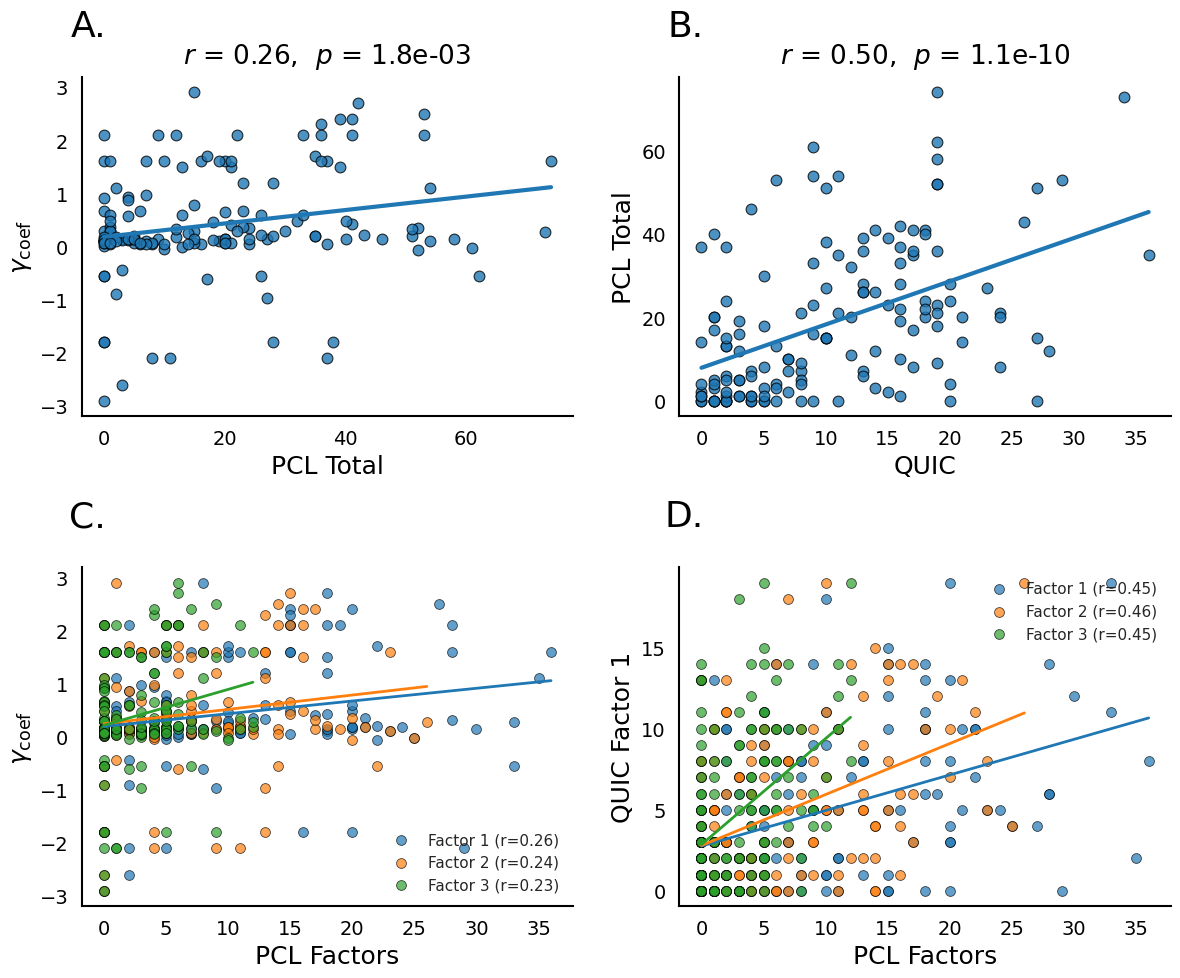
\includegraphics[width=0.8\linewidth]{figure5.png}
    \caption{\textbf{Dissociation between early-life unpredictability and PTSD symptoms in predicting uncertainty weighting.}
    (A) $\gamma_{\text{coef}}$ is positively correlated with PCL total.
    (B) PCL total is strongly correlated with QUIC total.
    (C) $\gamma_{\text{coef}}$ shows weak positive correlations with PCL-derived factors.
    (D) PCL-derived factors are moderately correlated with ELU Factor 1, indicating shared variance between trauma symptoms and early-life unpredictability.}
    \label{fig:elu_pcl_dissociation_top}
\end{figure}


\section*{Discussion}



% Leave blank for now


Stuff


\section*{Data Availability}

All data and analysis code can be found in the GitHub link:

\url{https://github.com/zyxl100/foraging_MQLP_2026}

\section*{Grants}

% Leave blank

Stuff


\section*{Disclosures}

No conflicts of interest, financial or otherwise, are declared by the authors.




\section*{Author Contributions}

% Leave blank
Stuff

\bibliographystyle{apalike}
\bibliography{foraging_references}

\nocite{}
\nocite{}
\nocite{}

\printbibliography

\end{document}